\documentclass[dvipsnames]{beamer}
\usepackage[utf8]{inputenc}
\usepackage{listings}
\usepackage{comment}
\usepackage{soul}
%\usepackage{ulem}
\usepackage{subfig}
\setul{}{1pt}
\usepackage[oldenum, olditem]{paralist}
%allow even smaller text
\newcommand\tinytiny{\fontsize{4pt}{3}\selectfont}

\makeatletter
\let\old@lstKV@SwitchCases\lstKV@SwitchCases
\def\lstKV@SwitchCases#1#2#3{}
\makeatother
\usepackage{lstlinebgrd}
\makeatletter
\let\lstKV@SwitchCases\old@lstKV@SwitchCases

\lst@Key{numbers}{none}{%
    \def\lst@PlaceNumber{\lst@linebgrd}%
    \lstKV@SwitchCases{#1}%
    {none:\\%
     left:\def\lst@PlaceNumber{\llap{\normalfont
                \lst@numberstyle{\thelstnumber}\kern\lst@numbersep}\lst@linebgrd}\\%
     right:\def\lst@PlaceNumber{\rlap{\normalfont
                \kern\linewidth \kern\lst@numbersep
                \lst@numberstyle{\thelstnumber}}\lst@linebgrd}%
    }{\PackageError{Listings}{Numbers #1 unknown}\@ehc}}
\makeatother


\graphicspath{{logos/}}

\usepackage{tikz}
\graphicspath{{4_5/figures/}}

%disclaimer for Sandia. uncomment and the whole blob goes away @ b80c116300122
%\def\sandid{SANDXXXX PE}

% \title{Performance Portability with Kokkos}
\title{Kokkos 4.5 Release Briefing}

%BAD misuse of author field
\author{New Capabilities}

\date{2024-12-10}

\usetheme{kokkos}

\newif\ifshort
\newif\ifmedium
\newif\iffull
\newif\ifnotoverview

\newcommand{\TutorialDirectory}{\texttt{Intro-Full}}
\newcommand{\ExerciseDirectory}[1]{\texttt{Exercises/#1/}}
\newcommand{\TutorialClone}{\texttt{Kokkos/kokkos-tutorials/\TutorialDirectory}}

\definecolor{darkgreen}{rgb}{0.0, 0.5, 0.0}
\definecolor{darkred}{rgb}{0.8, 0.0, 0.0}
\definecolor{orange}{rgb}{0.8, 0.33, 0.0}
\definecolor{purple}{rgb}{0.60, 0.20, 0.80}
\colorlet{bodyColor}{blue!20}
\colorlet{patternColor}{orange!30}
\colorlet{policyColor}{green!30}

% http://tex.stackexchange.com/questions/144448/color-a-text-line-in-a-code-lstlisting
\lstnewenvironment{code}[1][]%
{
  %with txfonts: OT1/txr/m/n/10
  %with default fonts: OT1/cmr/m/n/10
  %\fontfamily{cmr}\selectfont
  %\showthe\font
   \noindent
   \minipage{\linewidth}
   %\vspace{0.5\baselineskip}
   \lstset{mathescape, escapeinside={<@}{@>},
moredelim=**[is][{\btHL[fill=patternColor]}]{@pattern}{@pattern},
moredelim=**[is][{\btHL[fill=red!30]}]{@warning}{@warning},
moredelim=**[is][{\btHL[fill=policyColor]}]{@policy}{@policy},
moredelim=**[is][{\btHL[fill=bodyColor]}]{@body}{@body},
moredelim=**[is][{\btHL[fill=red!30]}]{@warning}{@warning},
moredelim=**[is][\color{black}]{@black}{@black},
moredelim=**[is][\color{blue}]{@blue}{@blue},
moredelim=**[is][\bf]{@bold}{@bold},
moredelim=**[is][\it]{@italic}{@italic},
moredelim=**[is][\color{boldblue}\bf]{@boldblue}{@boldblue},
moredelim=**[is][\color{red}]{@red}{@red},
moredelim=**[is][\color{green}]{@green}{@green},
moredelim=**[is][\color{gray}]{@gray}{@gray},
moredelim=**[is][\color{darkgreen}]{@darkgreen}{@darkgreen},
moredelim=**[is][\color{darkred}]{@darkred}{@darkred},
moredelim=**[is][\color{orange}]{@orange}{@orange},
moredelim=**[is][\color{purple}]{@purple}{@purple},
keywords={},
#1}
}
{
  \endminipage
  %\vspace{1.0\baselineskip}
}

\makeatletter
\newif\ifATOlinebackground
\lst@Key{linebackground}{\tiny}{\def\ATOlinebackground{#1}\global\ATOlinebackgroundtrue}
\makeatother

\lstnewenvironment{shell}[1][]{%
  \global\ATOlinebackgroundfalse
  \lstset{language=sh,%
    showstringspaces=false,
    aboveskip=0pt,
    frame=none,
    numbers=none,
    belowskip=2pt,
    breaklines=true,
    #1,
    }
  %\ifATOlinebackground
  \lstset{linebackgroundcolor={
    \ATOlinebackground
  }}
  %\fi
  }{}

\lstnewenvironment{cmake}[1][]{%
  \global\ATOlinebackgroundfalse
  \lstset{language=sh,%
    showstringspaces=false,
    aboveskip=0pt,
    frame=none,
    numbers=none,
    belowskip=2pt,
    breaklines=true,
    #1,
    }
  %\ifATOlinebackground
  \lstset{linebackgroundcolor={
    \ATOlinebackground
  }}
  %\fi
  }{}

\newcommand{\inlinecode}[1]{{\lstset{basicstyle=\ttfamily,keywordstyle={},showstringspaces=false}\lstinline$#1$}}
\newcommand{\inlineshell}[1]{{\lstset{basicstyle=\ttfamily,keywordstyle={},showstringspaces=false}\lstinline$#1$}}

\setbeamercolor{block title}{fg=white, bg=SandiaLightBlue}
\setbeamercolor{block body}{bg=lightgray}
\setbeamercolor{block title alerted}{fg=white, bg=SandiaRed}
\setbeamercolor{block body alerted}{bg=lightgray}



%\usepackage[texcoord,grid,gridunit=mm,gridcolor=red!10,subgridcolor=green!10]{eso-pic}
\usepackage[absolute,overlay]{textpos}





% http://tex.stackexchange.com/questions/8851/how-can-i-highlight-some-lines-from-source-code

\usepackage{pgf, pgffor}
\usepackage{listings}
\usepackage{lstlinebgrd} % see http://www.ctan.org/pkg/lstaddons

\makeatletter
%%%%%%%%%%%%%%%%%%%%%%%%%%%%%%%%%%%%%%%%%%%%%%%%%%%%%%%%%%%%%%%%%%%%%%%%%%%%%%
%
% \btIfInRange{number}{range list}{TRUE}{FALSE}
%
% Test in int number <number> is element of a (comma separated) list of ranges
% (such as: {1,3-5,7,10-12,14}) and processes <TRUE> or <FALSE> respectively

\newcount\bt@rangea
\newcount\bt@rangeb

\newcommand\btIfInRange[2]{%
    \global\let\bt@inrange\@secondoftwo%
    \edef\bt@rangelist{#2}%
    \foreach \range in \bt@rangelist {%
        \afterassignment\bt@getrangeb%
        \bt@rangea=0\range\relax%
        \pgfmathtruncatemacro\result{ ( #1 >= \bt@rangea) && (#1 <= \bt@rangeb) }%
        \ifnum\result=1\relax%
            \breakforeach%
            \global\let\bt@inrange\@firstoftwo%
        \fi%
    }%
    \bt@inrange%
}
\newcommand\bt@getrangeb{%
    \@ifnextchar\relax%
        {\bt@rangeb=\bt@rangea}%
        {\@getrangeb}%
}
\def\@getrangeb-#1\relax{%
    \ifx\relax#1\relax%
        \bt@rangeb=100000%   \maxdimen is too large for pgfmath
    \else%
        \bt@rangeb=#1\relax%
    \fi%
}

%%%%%%%%%%%%%%%%%%%%%%%%%%%%%%%%%%%%%%%%%%%%%%%%%%%%%%%%%%%%%%%%%%%%%%%%%%%%%%
%
% \btLstHL<overlay spec>{range list}
%
% TODO BUG: \btLstHL commands can not yet be accumulated if more than one overlay spec match.
%
\newcommand<>{\btLstHL}[2]{%
  \only#3{\btIfInRange{\value{lstnumber}}{#1}{\color{#2}\def\lst@linebgrdcmd{\color@block}}{\def\lst@linebgrdcmd####1####2####3{}}}%
}%
\makeatother






% http://tex.stackexchange.com/questions/15237/highlight-text-in-code-listing-while-also-keeping-syntax-highlighting
%\usepackage[T1]{fontenc}
%\usepackage{listings,xcolor,beramono}
\usepackage{tikz}

\makeatletter
\newenvironment{btHighlight}[1][]
{\begingroup\tikzset{bt@Highlight@par/.style={#1}}\begin{lrbox}{\@tempboxa}}
{\end{lrbox}\bt@HL@box[bt@Highlight@par]{\@tempboxa}\endgroup}

\newcommand\btHL[1][]{%
  \begin{btHighlight}[#1]\bgroup\aftergroup\bt@HL@endenv%
}
\def\bt@HL@endenv{%
  \end{btHighlight}%
  \egroup
}
\newcommand{\bt@HL@box}[2][]{%
  \tikz[#1]{%
    \pgfpathrectangle{\pgfpoint{1pt}{0pt}}{\pgfpoint{\wd #2}{\ht #2}}%
    \pgfusepath{use as bounding box}%
    \node[anchor=base west, fill=orange!30,outer sep=0pt,inner xsep=1pt, inner ysep=0pt, rounded corners=3pt, minimum height=\ht\strutbox+1pt,#1]{\raisebox{1pt}{\strut}\strut\usebox{#2}};
  }%
}
\makeatother



\usetikzlibrary{calc}
\usepackage{xparse}%  For \NewDocumentCommand

% tikzmark command, for shading over items
\newcommand{\tikzmark}[1]{\tikz[overlay,remember picture] \node (#1) {};}

\makeatletter
\NewDocumentCommand{\DrawBox}{s O{}}{%
    \tikz[overlay,remember picture]{
    \IfBooleanTF{#1}{%
        \coordinate (RightPoint) at ($(left |- right)+(\linewidth-\labelsep-\labelwidth,0.0)$);
    }{%
        \coordinate (RightPoint) at (right.east);
    }%
    \draw[red,#2]
      ($(left)+(-0.2em,0.9em)$) rectangle
      ($(RightPoint)+(0.2em,-0.3em)$);}
}

\NewDocumentCommand{\DrawBoxWide}{s O{}}{%
    \tikz[overlay,remember picture]{
    \IfBooleanTF{#1}{%
        \coordinate (RightPoint) at ($(left |- right)+(\linewidth-\labelsep-\labelwidth,0.0)$);
    }{%
        \coordinate (RightPoint) at (right.east);
    }%
    \draw[red,#2]
      ($(left)+(-\labelwidth,0.9em)$) rectangle
      ($(RightPoint)+(0.2em,-0.3em)$);}
}

\NewDocumentCommand{\DrawBoxWideBlack}{s O{}}{%
    \tikz[overlay,remember picture]{
    \IfBooleanTF{#1}{%
        \coordinate (RightPoint) at ($(left |- right)+(\linewidth-\labelsep-\labelwidth,0.0)$);
    }{%
        \coordinate (RightPoint) at (right.east);
    }%
    \draw[black,#2]
      ($(left)+(-\labelwidth,0.9em)$) rectangle
      ($(RightPoint)+(0.2em,-0.3em)$);}
}
\makeatother

\usetikzlibrary{positioning}

\usetikzlibrary{shapes}

\hypersetup{
    colorlinks=true,
    linkcolor=blue,
    filecolor=magenta,
    urlcolor=cyan,
}



\shorttrue
\mediumfalse
\fullfalse

\begin{document}

\begin{frame}
  \titlepage
\end{frame}


\begin{frame}[fragile]{Outline}

  \textbf{4.5 Release Highlights}

  \begin{itemize}
    \item{Organizational}
    \item{SequentialHostInit}
    \item{Feature Highlights}
    \item{General Enhancements}
    \item{Graphs Enhancements}
    \item{Backend updates}
    \item{Tuning changes demo}
    \item{Build system updates}
    \item{Deprecations and other breaking changes}
    \item{Bug Fixes}
  \end{itemize}

\end{frame}

\begin{frame}{Find More}

  \textbf{Online Resources}:

  \begin{itemize}
    \item \url{https://github.com/kokkos}:
          \begin{itemize}
            \item Primary Kokkos GitHub Organization
          \end{itemize}
    \item \url{https://github.com/kokkos/kokkos-tutorials/wiki/Kokkos-Lecture-Series}:
          \begin{itemize}
            \item{Slides, recording and Q\&A for the Full Lectures}
          \end{itemize}
    \item \url{https://kokkos.org/kokkos-core-wiki}:
          \begin{itemize}
            \item Wiki including API reference
          \end{itemize}
    \item \url{https://kokkosteam.slack.com}:
          \begin{itemize}
            \item Slack workspace for Kokkos.
            \item Please join: fastest way to get your questions answered.
            \item Can whitelist domains, or invite individual people.
          \end{itemize}
  \end{itemize}

\end{frame}

\begin{frame}[fragile]{Kokkos Usage}
  \textbf{Would like to strengthen community bonds and discoverability}

  \vspace{10pt}
  \textit{List of Applications and Libraries}
  \begin{itemize}
    \item Add your app to \url{https://github.com/kokkos/kokkos/issues/1950}
    \item We are planning to add that to a Kokkos website.
    \item Helps people discover each other when working on similar things.
  \end{itemize}

  \vspace{10pt}
  \textit{GitHub Topics}
  \begin{itemize}
    \item Use \textit{kokkos} tag on your repos.
    \item If you click on the topic you get a list of all projects on github with that topic.
  \end{itemize}
\end{frame}


%==========================================================================

\begin{frame}[fragile]

  {\Huge Organizational}

  \vspace{10pt}

  \textbf{Content:}
  \begin{itemize}
    \item HPSF and Kokkos Meeting 2025
    \item Targeting C++20 for Kokkos 5.0
    \item Makefile deprecation
  \end{itemize}

\end{frame}

%==========================================================================

\begin{frame}[fragile]{Kokkos User Group Meeting 2025}
\begin{center}
\textbf{Kokkos User Group Meeting 2025 @ HPSF Conference}
\end{center}

\begin{itemize}
\item{\textit{When:} May 5th-8th 2025}
\item{\textit{Where:} Chicago}
\item{\textit{What:} 2-days HPSF plenary + 2-days Project meetings}
\item{\textit{KUG-Content:} Focused on user experiences
\begin{itemize}
   \item{How do you leverage Kokkos?}
   \item{What are pain points?}
   \item{Kokkos-based libraries of interest to the community}
\end{itemize}
}
\end{itemize}

\vspace{10pt}

\begin{center}
\textit{Registration open now!}
\end{center}
\end{frame}

\begin{frame}[fragile]{Kokkos User Group Meeting 2025}
\begin{center}
\textbf{What to expect from KUG}
\end{center}

\begin{itemize}
  \item{Eight 90-minute sessions featuring a dynamic blend of Kokkos developers and community users}

  \begin{multicols}{2}
    \item{\textit{Day 1 Highlights:}}
      \begin{itemize}
        \item{Essential Updates}
        \item{Kokkos in Applications}
        \item{Adopting Kokkos}
        \item{Lightning Talks}
    \end{itemize}

    \columnbreak

    \item{\textit{Day 2 Highlights:}}
      \begin{itemize}
        \item{Kokkos Ecosystem}
        \item{Tuning and Performance}
        \item{Algorithms}
        \item{Panel Discussion}
    \end{itemize}
  \end{multicols}
\end{itemize}
\end{frame}

\begin{frame}[fragile]{HPSF Conference 2025}
\begin{center}
\textbf{Other reasons to go}
\end{center}

\begin{itemize}
  \item{General Poster Session}
  \item{Updates on the HPSF project}
  \item{Introduction to various working groups}
  \item{Various Panel Discussions}
  \item{Chance to meet all other members of HPSF}
  \item{...}
\end{itemize}
\end{frame}

\begin{frame}[fragile]{Other outreach}
  \begin{itemize}
    \item{HPSF will be present at \href{https://isc.app.swapcard.com/widget/event/isc-high-performance-2025/planning/UGxhbm5pbmdfMjU4NjE0MQ==}{ISC BOF 2025}}
\item{\href{https://kokkos.org/community/tea-time/}{Kokkos Tea-Time} on 2nd or 3rd Wed of the month} 
  \begin{itemize}
      \item April 16th @ 11am EST "Solomon: unified schemes for directive-based GPU offloading"
  \end{itemize}
\end{itemize}

\end{frame}


\begin{frame}[fragile]{Kokkos 5 and ISO C++20}
\begin{center}
\textbf{Kokkos 5 is comming Summer 2025}

\vspace{0.5cm}
\textbf{We will require C++20!}
\end{center}

\textit{Start preparing now:}
\begin{itemize}
  \item{Check availability of compilers on your systems}
  \item{Test with C++20 enabled: start with a CPU build}
  \item{Minimum Compiler requirements will change (more details later)}
\end{itemize}

\vspace{0.5cm}
\begin{center}
\textit{Nothing wrong for your project to require C++20 now if you feel ready!}
\end{center}
\end{frame}

\begin{frame}[fragile]{Makefile deprecation}
\begin{center}
\textbf{Makefile is officially deprecated and will be removed in the next major release}

\textit{Start preparing now:}
\begin{itemize}
  \item{Check if you can transition to CMake}
  \item{Comment on pinned issue \href{https://github.com/kokkos/kokkos/issues/7610}{7610}}
\end{itemize}
\end{center}

\end{frame}

\begin{frame}[fragile]{Open SSF Scorecard}
\begin{center}
\textbf{We reached ``passed'' on the OSSF Best Practices Program}
\href{https://www.bestpractices.dev/en/projects/9344}{www.bestpractices.dev}

\vspace{0.5cm}
\textit{This means Kokkos is continuously tracking and openly reporting the conformity with open source software practices.}
\end{center}

\end{frame}

%==========================================================================

\begin{frame}[fragile]

  {\Huge SequentialHostInit and Views of Views}
  
    \vspace{10pt}
\begin{center}
\textit{Or:} What to do if you need Views of "complicated" objects?
\end{center}

\end{frame}

%==========================================================================

\begin{frame}[fragile]{"Complicated" objects}
\textbf{To create a \textit{normal} \texttt{View} the objects it views need to be:}
\begin{itemize}
  \item default-constructible in the View associated execution space
  \item destructible in the View associated execution space 
\end{itemize}

\vspace{10pt}

\textbf{This Means:} Default constructor and desctructor:
\begin{itemize}
\item{must be \texttt{KOKKOS\_FUNCTION} (or defaulted)}
\item{can't allocate or deallocate data}
\item{can't call Kokkos parallel operations (\texttt{parallel\_for} etc.)}
\item{can't create or destroy Views!}
\end{itemize}

\vspace{10pt}
\begin{center}
\textit{If your object does any of these things it is "Complicated"!}
\end{center}

\end{frame}

%==========================================================================

\begin{frame}[fragile]{SequentialHostInit view allocation property in 4.5}

\begin{itemize}
\item Construction and Destruction of objects will happen sequentially on Host!
\item Backported to 4.4.1
\end{itemize}

\begin{code}
using Complicated = Kokkos::View<T*, SomeMemorySpace>
View<Complicated**, HostSpace> v(view_alloc("v", SequentialHostInit), 2, 3);
// copy assign elements
v(0,0) = Complicated("w00", 4);
v(1,0) = Complicated("w10", 5);
v(0,1) = Complicated("w01", 6);
// v.~View() handles properly elements destruction
\end{code}

\vspace{10pt}
\textbf{Requirements for generic "Complicated" types:}
\begin{itemize}
\item \texttt{T} is default constructible and destructible on host
\item \texttt{SomeMemorySpace} is host accessible (e.g. \texttt{SharedSpace} or \texttt{HostSpace})
\end{itemize}
\end{frame}

%==========================================================================

\begin{frame}[fragile]{How do I know I need this?}
\begin{center}
Since Kokkos 4.4 programs may dead-lock when creating or destroying View's of complicated objects!
\end{center}

\vspace{10pt}

Previously legal code leveraging `WithoutInitializing` with proper element clean-up before destruction continues to be legal!
\end{frame}
%==========================================================================



%==========================================================================

\begin{frame}[fragile]

  {\Huge Feature highlights}

  \vspace{10pt}

\end{frame}

%==========================================================================

% Examples

% note: always keep the [fragile] for your frames!

%\begin{frame}[fragile]{Example list}
%  \begin{itemize}
%      \item Item 1
%      \item Item 2 with some \texttt{code}
%      \begin{itemize}
%        \item Sub-item 2.1
%        \item Sub-item 2.2
%      \end{itemize}
%  \end{itemize}
%\end{frame}

%\begin{frame}[fragile]{Example code}
%    \begin{code}[keywords={std}]
%        #include <iostream>
%        
%        int main() {
%            std::cout << "hello world\n";
%        }
%    \end{code}
%\end{frame}

%\begin{frame}[fragile]{Example table}
%    \begin{center}
%        \begin{tabular}{l|l}
%            a & b \\\hline
%            c & d
%        \end{tabular}
%    \end{center}
%\end{frame}

%==========================================================================

% \begin{frame}[fragile]\label{sec:new_features}

  % {\Huge Kokkos::Graph features}

  % \vspace{10pt}

% \end{frame}

\begin{frame}[fragile]{Kokkos::Graph recap}
 \begin{itemize}
     \item describes asynchronous workloads organised as a direct acyclic graph (DAG)
     \item executed using \texttt{submit()}, possibly many times, observing dependencies
      \begin{code}[keywords={auto}]
auto graph = Kokkos::create_graph([&](auto root) {
    auto node_A = root.then_parallel_for("A", ...policy..., ...functor...);
    auto node_B = node_A.then_parallel_for("B", ...policy..., ...functor...);
    auto node_C = node_A.then_parallel_for("C", ...policy..., ...functor...);

    auto node_D = Kokkos::when_all(node_B, node_C).
                  then_parallel_for("D", ...policy..., ...functor...);
});

graph.instantiate();

graph.submit();
      \end{code}
 \end{itemize}
\end{frame}

\begin{frame}[fragile]{Kokkos::Graph new features}
 \begin{itemize}
  \item \texttt{then} node: executes a callable on device
  \item Single call of the functor per \texttt{submit()}
   \item Executed in the \texttt{ExecutionSpace} the graph is submitted to
     \begin{code}[keywords={auto}]
auto graph = Kokkos::create_graph([&](auto root) {
    auto node_A = root.then_parallel_for("A", ...policy..., ...functor...);
    auto node_B = node_A.then("B", ...functor...);
});   
     \end{code}
   \item Functor passed to \texttt{then} must be callable without arguments and marked with \texttt{KOKKOS\_FUNCTION}
 \end{itemize}
\end{frame}

\begin{frame}[fragile]{Kokkos::Graph new features}
 \begin{itemize}
   \item Interoperability: create a \texttt{Kokkos::Graph} from a native Cuda/HIP/Sycl graph
     \begin{code}[keywords={create_graph_from_native}]
cudaGraph_t native_graph = nullptr;
cudaGraphCreate(&native_graph, 0);

auto graph_from_native =
  Kokkos::Experimental::create_graph_from_native(exec, native_graph);
     \end{code}
    \item Experimental, does not yet allow adding nodes created using the native API to a \texttt{Kokkos::Graph}
 \end{itemize}
\end{frame}

% \begin{frame}[fragile]\label{sec:new_features}

  % {\Huge Multi-GPU for HIP Backend}

  % \vspace{10pt}

% \end{frame}

\begin{frame}[fragile]{Multi-GPU for HIP Backend}
  \begin{itemize}
    \item Launch kernels on multiple devices from a single host process
    \item Available for ROCm 5.6 and later
    \item Requires direct use of HIP runtime API for creating and destroying streams
    \item Experimental, still looking for feedback from new users
    \item New documentation (for all backends)  
      \begin{itemize} 
        \item[] \url{https://kokkos.org/kokkos-core-wiki/API/core/MultiGPUSupport.html}
      \end{itemize}
  \end{itemize}
\end{frame}

\begin{frame}[fragile]{Multi-GPU for HIP Backend}
  \begin{code}[keywords={auto}]
// Create streams on different devices
hipStream_t streams[2];
hipSetDevice(0); hipStreamCreate(&streams[0]);
hipSetDevice(1); hipStreamCreate(&streams[1]);
{
  // Creating execution spaces 
  Kokkos::HIP exec0(streams[0]), exec1(streams[1]);

  // Allocating views
  Kokkos::View<int*> v0(Kokkos::view_alloc("v0", exec0), N);
  Kokkos::View<int*> v1(Kokkos::view_alloc("v1", exec1), M);

  // Launch kernels (run concurrently)
  Kokkos::parallel_for(Kokkos::RangePolicy(exec0, 0, N), functor0);
  Kokkos::parallel_for(Kokkos::RangePolicy(exec1, 0, M), functor1);
}
// Destroy streams (after execution spaces are deleted)
hipStreamDestroy(streams[0]); hipStreamDestroy(streams[1]);
  \end{code}
\end{frame}

%==========================================================================

%==========================================================================

\begin{frame}[fragile]

  {\Huge General Enhancements}
  
    \vspace{10pt}

\end{frame}

%==========================================================================

%==========================================================================

\begin{frame}[fragile]

  {\Huge Graphs Enhancements}

  \vspace{10pt}

\end{frame}

%==========================================================================

% Merged GitHub PR with 2 arguments:
%  - PR number
%  - PR title
\newcommand{\mergedPR}[2]{
    \item \href{https://github.com/kokkos/kokkos/pull/#1}{#2}
}

\usetikzlibrary{positioning}

\begin{frame}[fragile]{Graphs Enhancements: Basics (1/5)}

  \texttt{Kokkos::Graph} is an asynchronous execution model that requires all workloads
  to be defined ahead of execution - as opposed to \emph{eager} execution that you get with
  a regular execution space instance.

  \vspace{1em}

  \begin{columns}
    \centering
    \begin{column}{0.25\textwidth}
      \centering
      \begin{tikzpicture}[
        main node/.style = {circle, fill = blue!20, draw, minimum size = 0.75cm, inner sep = 0pt}
      ]  

        \node[main node, fill=SandiaLightLightBlue] (A) at ( 0   ,  0) {$A$};
        \node[main node, fill=SandiaLightLightBlue] (B) at (-1   , -1) {$B$};
        \node[main node, fill=SandiaLightLightBlue] (C) at (-1.75, -2) {$C$};
        \node[main node, fill=SandiaLightLightBlue] (D) at (-0.25, -2) {$D$};
        \node[main node, fill=SandiaLightLightBlue] (E) at (-1   , -3) {$E$};
        \node[main node, fill=SandiaLightLightBlue] (X) at ( 1   , -1) {$X$};
        \node[main node, fill=SandiaLightLightBlue] (Y) at ( 1   , -2) {$Y$};

        \path[draw,thick] (A) edge node {} (B);
        \path[draw,thick] (A) edge node {} (X);
        \path[draw,thick] (B) edge node {} (C);
        \path[draw,thick] (B) edge node {} (D);
        \path[draw,thick] (C) edge node {} (E);
        \path[draw,thick] (D) edge node {} (E);
        \path[draw,thick] (X) edge node {} (Y);

      \end{tikzpicture}
    \end{column}%
    \begin{column}{0.75\textwidth}
      \centering
      \begin{block}{}
        \begin{itemize}
          \item Makes your code semantics clear and portable.
          \item Reduces CPU overhead due to scheduling (\texttt{Cuda} and {\texttt{HIP}}).
          \item Enables as many compiler/driver optimizations as possible.
        \end{itemize}
      \end{block}
    \end{column}
  \end{columns}

\end{frame}

\begin{frame}[fragile]{Graphs Enhancements: PRs (2/5)}

  Main PRs for the current release that modified \texttt{Kokkos::Graph}
  \begin{itemize}
    \mergedPR{7240}{core(graph): \textbf{promote instantiate} to public API}
    \mergedPR{7249}{core(graph): allow submission onto an \textbf{arbitrary exec} space instance}
    \mergedPR{7271}{graph(fix): \textbf{defaulted graph submit} control flow}
    \mergedPR{7248}{core(graph): allow \textit{create\_graph} \textbf{without closure}}
    \mergedPR{6904}{graph: allow access to \textbf{native graph} object}
    \mergedPR{7460}{graph(diagnostic): enable compile-time diagnostic of \textbf{illegal reduction target}}
    \mergedPR{7365}{graph(global-kernel-launch): fix global launch for node kernel}
  \end{itemize}

\end{frame}

\begin{frame}[fragile]{Graph Enhancements (3/5)}

  \begin{itemize}
    \item Using a \texttt{Kokkos::Graph} is a 3-phase process
          \begin{enumerate}
            \item Definition
            \item Instantiation
            \item Submission
          \end{enumerate}

    \item \texttt{Kokkos} will instantiate the graph on the first \texttt{submit} if needed.

    \item \texttt{Kokkos} will \texttt{submit} the graph on the execution space instance provided
  during \emph{definition} by default.
  \end{itemize}

  \begin{code}
    auto graph = Kokkos::Experimental::create_graph<...>(exec,
        [&](const auto& root) {... /* add nodes */ ...});

    graph.instantiate(); // optional

    graph.submit(/* other_exec */);
  \end{code}

\end{frame}

\begin{frame}[fragile]{Graph Enhancements (4/5)}

  Then...

  \begin{code}
    auto graph = Kokkos::Experimentalcreate_graph<Kokkos::HIP>(
      exec, [&](const auto& root) {
        auto node = root.then_parallel_...;
    });
  \end{code}

  Now...

  \begin{itemize}
    \item \texttt{Kokkos} now allows graph \emph{definition} outside of a closure.

    \item \texttt{Kokkos} allows access to the underlying backend graph (\texttt{hipGraph\_t} and so on).
  \end{itemize}

  \begin{code}
    auto graph = Kokkos::Experimental::create_graph<Kokkos::HIP>(exec);
    // Impl shall disappear at some point.
    auto root  = Kokkos::Impl::GraphAccess::create_root_ref(graph);
    auto node  = root.then_parallel_...;

    size_t num_nodes;
    hipGraphGetNodes(graph.native_graph(), nullptr, &num_nodes);
  \end{code}

\end{frame}

\begin{frame}[fragile]{Graph Enhancements (5/5)}

  \begin{itemize}
    \item The defaulted graph implementation received some attention (\emph{exec} correctness), but can still be
          enhanced.
    \item Kernels nodes with global launch were fixed (\texttt{HIP} and \texttt{Cuda}).
    \item Better compile-time diagnostic for illegal reduction target. It must be device-accessible.
  \end{itemize}

\end{frame}


%==========================================================================

\begin{frame}[fragile]

  {\Huge Backend Updates}

  \vspace{10pt}

  \textbf{Content:}
  \begin{itemize}
    \item SYCL
    \item OpenMPTarget
    \item CUDA and HIP
  \end{itemize}

\end{frame}

%==========================================================================

\begin{frame}[fragile]{SYCL Backend Updates}
\begin{itemize}
\item For \texttt{RangePolicy} with \texttt{parallel\_for}, the workgroup size can be specified manually:
\begin{code}
parallel_for(
  RangePolicy<ExecutionSpace>(space, 0, N)
    .set_chunk_size(1024), *this);
\end{code}

\item Intel compiler flags very aggressive, applications might need
\begin{code}
-fp-model=precise
\end{code}

or similar for correct results.
\end{itemize}
\end{frame}

%==========================================================================


\begin{frame}[fragile]{OpenMPTarget Backend Updates}

    \begin{itemize}
        \item The backend now allows selecting the default GPU which can be set by using \texttt{--kokkos-device-id=<number>}. 
        \item The backend can now detect the number of devices on a single node. 
    \end{itemize}
    
\end{frame}
 
%==========================================================================

\begin{frame}[fragile]{CUDA Backend Updates}
  \begin{itemize}
    \item Allow CUDA PTX forward compatibility 
      \begin{itemize}
        \item code compiled for compute capability 5.2 will now run on device compute capability 7.5
      \end{itemize}
    \item Improve CUDA cache config setting
      \begin{itemize}
        \item let CUDA runtime decide what is the best usage of the cache (shared vs L1 balance)
      \end{itemize}
    \item Do not rely on synchronization behavior of default stream
      \begin{itemize}
        \item default instance does not synchronize the other instances
      \end{itemize}
    \item Add support for Hopper architecture
  \end{itemize}
\end{frame}

%==========================================================================

\begin{frame}[fragile]{HIP Backend Updates}
  \begin{itemize}
    \item HIP, HIPSpace, HIPHostPinnedSpace, and HIPManagedSpace out of
      Experimental
      \begin{itemize}
        \item backward compatible change
        \item long term support of ROCm 5.2 and later
      \end{itemize}
    \item Export AMD architecture flags when using Trilinos
      \begin{itemize}
        \item fix issue when compiling on node without GPU
      \end{itemize}
    \item Do not rely on synchronization behavior of default stream
    \item Dropped support for MI25 and added support for Navi1030
  \end{itemize}
\end{frame}

%==========================================================================

\begin{frame}[fragile]{HIP Backend Updates}
  \begin{itemize}
    \item There is a compiler bug ROCm 5.3 and 5.4 when using LocalMemory launch mechanism: 
      \begin{itemize}
        \item sometimes hangs
        \item sometimes passes
        \item often error out with \emph{Reason: Unknown}
      \end{itemize}
    \item To fix the issue, force GlobalMemory launch mechanism
\begin{code}[keywords={ImplForceGlobalLaunch}]
parallel_for(
  Experimental::require(
    RangePolicy(0, N),
    Experimental::WorkItemProperty::ImplForceGlobalLaunch),
  ...);
\end{code}
    \item We do not apply unconditionally because it reduces performance
  \end{itemize}
\end{frame}

%==========================================================================

\begin{frame}[fragile]{Bug fixes for CUDA and HIP Backends}
  \begin{itemize}
     \item CUDA and HIP fixes:
       \begin{itemize}
         \item Fix incorrect offset when using parallel\_scan for $<$ 4 bytes data
           types
         \item Fix max scratch size calculation for level 0 scratch
       \end{itemize}
     \item HIP fixes:
       \begin{itemize}
         \item Fix linking error when using amdclang (OLCFDEV-1167)
         \item Fix race condition when using \texttt{HSA\_XNACK=1}
       \end{itemize}
  \end{itemize}
\end{frame}

%==========================================================================

\begin{frame}[fragile]{Default instance synchronization behavior}
  \begin{itemize}
  \item CUDA and HIP default instances used to implicitly synchronize with other instances as well as raw CUDA and HIP code
  \item This was NOT intentional behavior
\begin{code}
parallel_for(N, f1);
// f2 would be sequenced after f1 in previous releases
parallel_for(RangePolicy<>(exec, 0 , N), f2);
\end{code}
  \item Call \texttt{DefaultExecutionSpace().fence()}
  \item Beware of non-Kokkos code calling CUDA or HIP
    \begin{itemize}
    \item MPI, BLAS, etc.
    \item Previously might have been implicitly synchronized with Kokkos code
    \end{itemize}
  \end{itemize}
\end{frame}

%==========================================================================

\begin{frame}[fragile]

  {\Huge Tuning Changes Demo}

  \vspace{10pt}

\end{frame}

%==========================================================================

% Examples

% note: always keep the [fragile] for your frames!

\begin{frame}[fragile]{Kokkos Runtime Tuning Overview/Review (1/7)}
  \begin{itemize}
      \item Kokkos has runtime auto-tuning support when configured with
      \begin{itemize}
        \item \texttt{Kokkos\_ENABLE\_TUNING} CMake variable enabled at configuration time
      \end{itemize}
      \item Kokkos internal auto-tuning support is enabled at runtime when
      \begin{itemize}
        \item \texttt{--kokkos-tune-internals} command line variable enabled at run time
        \item a Kokkos tool is used to provide the search
      \end{itemize}
      \item Internal tunable parameters (available before 4.5)
      \begin{itemize}
        \item \texttt{MDRangePolicy} - $X$, $Y$, $Z$ block sizes for CUDA, HIP execution spaces
        \item \texttt{TeamPolicy} - team size and vector length for CUDA, HIP execution spaces
      \end{itemize}
      \item Arbitrary runtime parameters can be tuned with the same API, code modifications required - we hope to simplify (or abstract) that API
  \end{itemize}
\end{frame}

\begin{frame}[fragile]{Kokkos Runtime Tuning New Features (2/7)}
  \begin{itemize}
      \item New Internal tunable parameters (4.5)
      \begin{itemize}
        \item \texttt{RangePolicy} - Occupancy (with code modification) for CUDA execution space
        \item \texttt{MDRangePolicy} - Occupancy (with code modification) for CUDA execution space
        \item \texttt{TeamPolicy} - Occupancy (with code modification) for CUDA execution space
      \end{itemize}
      \item Occupancy value tuned between [5:100], step size of 5
      \item Natural extension of PR \#3379: ``Experimental feature: control cuda occupancy''
      \begin{block}{}
          \textit{``...passing \texttt{prefer(policy, DesiredOccupancy(33))} to a \texttt{parallel\_for()}, \texttt{parallel\_reduce()}, or \texttt{parallel\_scan} will bypass the block size deduction that tries to maximize the occupancy and adjust the launch parameters (by fixing the block size and requesting shared memory) to achieve the specified occupancy. The desired occupancy is in percent.''}
      \end{block}
  \end{itemize}
\end{frame}

\begin{frame}[fragile]{Occupancy Example - code change required (3/7)}
    \begin{code}[keywords={std}]
    using memory_space = typename Kokkos::DefaultExecutionSpace::memory_space;
    using view_type = Kokkos::View<double **, memory_space>;
    view_type left("process_this", 1000000, 25);
    /* Create a policy wrapper to request a tuned occupancy value from 0-100 */
    auto const occupancy_policy = Kokkos::Experimental::prefer(
        Kokkos::RangePolicy<>(0, left.extent(0)),
        Kokkos::Experimental::DesiredOccupancy{Kokkos::AUTO});
    const auto kernel = KOKKOS_LAMBDA(int i) {
            for (int r = 0; r < 25; r++) {
                double f = 0.;
                for (int m = 0; m < left.extent_int(1); m++) {
                    f += left(i, m);
                    left(i, m) += f;
                }
            }
        };
    Kokkos::parallel_for("Bench", occupancy_policy, kernel);
    \end{code}
\end{frame}

\begin{frame}[fragile]{APEX Auto-tuning Support (4/7)}
  \begin{itemize}
      \item APEX 2.7.0 released: \url{https://github.com/UO-OACISS/apex}
      \item Included as git submodule in kokkos-tools: \url{https://github.com/kokkos/kokkos-tools/tree/develop/tpls/apex}
      \item Profiling and tracing support for both asynchronous tasking runtimes and ``conventional'' parallel models (MPI, OpenMP, OpenACC, OpenCL, CUDA, HIP, SYCL, Kokkos, Pthreads, HPX, PaRSEC, StarPU, Iris...)
      \item Runtime adaptation search strategies (exhaustive, random, simulated annealing, genetic search, nelder mead, auto) integrated with Kokkos tuning API
      \item Growing set of example cases: \url{https://github.com/khuck/apex-kokkos-tuning}
      \item Long article on Kokkos autotuning with APEX: \url{https://github.com/UO-OACISS/apex/wiki/Kokkos-Runtime-Auto-Tuning-with-APEX}
  \end{itemize}
\end{frame}

\begin{frame}[fragile]{Running with APEX (5/7)}
    \begin{code}[keywords={bash}]
# Specify the search strategy
export APEX_KOKKOS_TUNING_POLICY=nelder_mead
# Specify the number of samples to be taken for each configuration
export APEX_KOKKOS_TUNING_WINDOW=4
# Run with apex_exec
apex_exec --apex:kokkos-tuning ./occupancy_example --kokkos-tune-internals

# Possible (truncated) verbose output:
...
Nelder Mead: New best! 0.00197833 k: 1, Bench: 30
Nelder Mead: New best! 0.00196357 k: 7, Bench: 20
Nelder Mead: New best! 0.00196042 k: 10, Bench: 25
Nelder Mead: New best! 0.00195894 k: 48, Bench: 25
...
Converged after 43 iterations.
Total func evaluations: 114
APEX: Tuning has converged for session 1.
[25]

    \end{code}
\end{frame}

\begin{frame}[fragile]{Perfetto trace of example tuned by APEX for Nelder Mead search strategy (6/7)}
    \begin{center}
    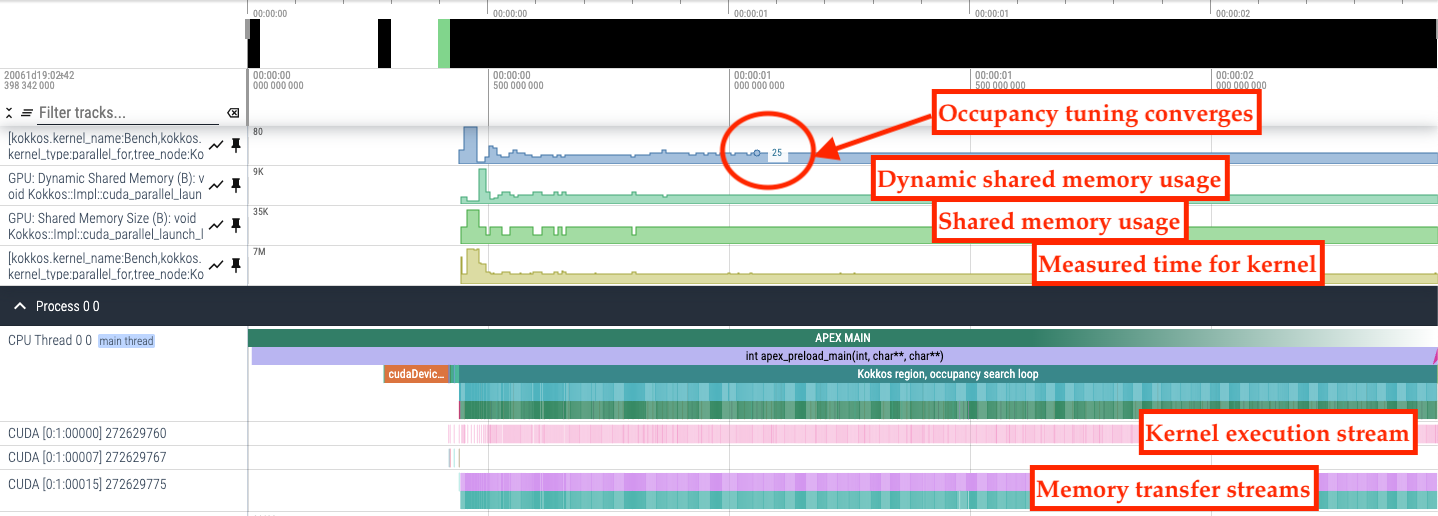
\includegraphics[width=\linewidth]{4_5/tuning/nelder_mead_occupancy_trace.png}
    \end{center}
\end{frame}

\begin{frame}[fragile]{Kokkos Potential Future Tuning Plans (7/7)}
  \begin{itemize}
      \item Simplified/abstracted API for custom tuning in user code (or at least some helper functions)
      \begin{itemize}
        \item \texttt{kokkosp\_declare\_[input,output]\_type} - make it easier to create variables
        \item \texttt{kokkosp\_[begin,end]\_context}
        \item \texttt{kokkosp\_request\_values}
      \end{itemize}
      \item Additional examples, performance studies
      \item Internal tuning for \texttt{RangePolicy}
      \item Internal support/testing for more execution engines (SYCL, OpenMP, OpenMPTarget)
  \end{itemize}
\end{frame}

%==========================================================================

%==========================================================================

\begin{frame}[fragile]

  {\Huge Build Systems Updates}

  \vspace{10pt}

\end{frame}

%==========================================================================

% Examples

% note: always keep the [fragile] for your frames!

\begin{frame}[fragile]{New build system features}
  \begin{itemize}
    \item Add support for Zen 4 AMD microarchitecture (\texttt{Kokkos\_ARCH\_ZEN4})
    \item Enable NVIDIA Grace architecture with NVHPC (\texttt{Kokkos\_ARCH\_ARMV9\_GRACE})
    \item Support static library builds via \texttt{CMAKE\_CUDA\_RUNTIME\_LIBRARY=static} when using CUDA as CMake language
  \end{itemize}

\end{frame}

%==========================================================================

\begin{frame}[fragile]{Spack support for MI300A}
  \begin{itemize}
    \item Spack \textit{develop} branch now supports MI300A with a new variant \textcolor{red}{\texttt{apu}}
    (\href{https://github.com/spack/spack/pull/48609}{spack/spack\#48609})

    \item To compile Kokkos for MI300A, forcing the APU mode, use the following command:
    \texttt{spack install kokkos +rocm amdgpu\_target=gfx942 \textcolor{red}{+apu}}

    % In pure CMake, this is equivalent to:
    % cmake -DKokkos_ENABLE_ROCM=ON -DKokkos_ARCH_AMD_GFX942_APU=ON
  \end{itemize}

\end{frame}


%==========================================================================

%==========================================================================

\begin{frame}[fragile]

  {\Huge Deprecations and other breaking changes}

  \vspace{10pt}

\end{frame}


\begin{frame}[fragile]{Dropping support for Intel C++ Compiler Classic}
  \begin{itemize}
    \item Intel has deprecated Intel Classic in 2022, and removed it from oneAPI 2024
    \item In order to focus on newer compilers, and reduce maintenance burden, we have \textbf{removed} support for Intel Classic (oneAPI Intel/icpx still supported of course!)
  \end{itemize}
\end{frame}


\begin{frame}[fragile]{DualView changes}
  \textbf{Deprecate} direct access to \texttt{d\_view} and \texttt{h\_view}
  \begin{itemize}
    \item Modifying the allocations in d\_view and h\_view directly is dangerous, especially if \texttt{modify} and \texttt{sync} are skipped
    \item Use \texttt{view\_host()} and \texttt{view\_device()} instead
    \item These two functions return by value with deprecated code enabled and by const reference otherwise. This might have perfomance implications if used extensively, e.g., in loop bounds.
  \end{itemize}
\end{frame}


\begin{frame}[fragile]{Experimental SIMD changes}
  \begin{itemize}
    \item \texttt{native\_simd}, \texttt{native\_simd\_mask} \textbf{deprecated} to align with the C++26 standard
    \item \textbf{Removed} Obtaining a reference from SIMD \texttt{operator[]} to align with the C++26 Standard
    \item \textbf{Changed} the return type of SIMD \texttt{operator==} and \texttt{operator!=} to return SIMD masks instead of \texttt{bool}
    \begin{itemize}
      \item If you want old behavior, use \texttt{all\_of(a == b)}
    \end{itemize}
  \end{itemize}
\end{frame}

\begin{frame}[fragile]{Additional Deprecations and Removals}
  \begin{itemize}
    \item Already discussed deprecating the Makefile
    \item StaticCrsGraph is \textbf{moved} to Kokkos Kernels and \textbf{deprecated} in Core
    \begin{itemize}
      \item See \url{https://github.com/kokkos/kokkos-kernels/pull/2419}
      \item Symbol is in Kernels under \texttt{KokkosSparse::StaticCrsGraph}
    \end{itemize}
  \end{itemize}
\end{frame}
%==========================================================================

% Examples

% note: always keep the [fragile] for your frames!

%\begin{frame}[fragile]{Example list}
%  \begin{itemize}
%      \item Item 1
%      \item Item 2 with some \texttt{code}
%      \begin{itemize}
%        \item Sub-item 2.1
%        \item Sub-item 2.2
%      \end{itemize}
%  \end{itemize}
%\end{frame}

%\begin{frame}[fragile]{Example code}
%    \begin{code}[keywords={std}]
%        #include <iostream>
%        
%        int main() {
%            std::cout << "hello world\n";
%        }
%    \end{code}
%\end{frame}

%\begin{frame}[fragile]{Example table}
%    \begin{center}
%        \begin{tabular}{l|l}
%            a & b \\\hline
%            c & d
%        \end{tabular}
%    \end{center}
%\end{frame}

%==========================================================================


%==========================================================================


%==========================================================================

\begin{frame}[fragile]

        {\Huge Further Deprecations in Release 3.7}

  \vspace{-20pt}

\end{frame}

%==========================================================================

\begin{frame}[fragile]{Removing \texttt{finalize\_all}}

\begin{itemize}
\item Deprecated \texttt{Kokkos::finalize\_all()}
\item Use \texttt{Kokkos::finalize()} instead
\end{itemize}

\end{frame}

%==========================================================================

\begin{frame}[fragile]{\texttt{volatile} overload of \texttt{Reducer::join}}
\textbf{Non-\texttt{volatile} member function called}
\begin{code}[keywords={volatile}]
struct DeprecatedReducer {  // just happened to work
  KOKKOS_FUNCTION
  void join(value_type volatile& dst,
            value_type const volatile& src) const;
};

struct Release37AndBeyondReducer {
  KOKKOS_FUNCTION
  void join(value_type& dst,
            value_type const& src) const;
};

struct BackwardCompatibleReducer {
  KOKKOS_FUNCTION
  void join(value_type& dst,
            value_type const& src) const;
  KOKKOS_FUNCTION
  void join(value_type volatile& dst,
            value_type const volatile& src) const;
};
\end{code}

\end{frame}

%==========================================================================

\begin{frame}[fragile]{Public/private headers}
\textbf{Compilation error when including private Kokkos headers}

{\tiny
\begin{verbatim}
<kokkos>/core/src/Kokkos_View.hpp:47:1: error: static_assert failed
  "Including non-public Kokkos header files is not allowed."
static_assert(false,
^             ~~~~~
1 error generated.
\end{verbatim}
}

\begin{itemize}
\item See \href{https://github.com/kokkos/kokkos/issues/4856}{GitHub Issue \#4856}
\item Why can't I just include \texttt{<Kokkos\_View.hpp>} or \texttt{<Kokkos\_Parallel.hpp>}
\end{itemize}


\tiny
\begin{tabular}{ll}
Symbol & header \texttt{\#include} \\
\texttt{Kokkos::View}          & \texttt{<Kokkos\_Core.hpp>} \\
\texttt{Kokkos::parallel\_for} & \texttt{<Kokkos\_Core.hpp>} \\
\texttt{Kokkos::fence}         & \texttt{<Kokkos\_Core.hpp>} \\
\texttt{KOKKOS\_FUNCTION}      & \texttt{<Kokkos\_Core.hpp>} or \texttt{<Kokkos\_Macros.hpp>} \\
\texttt{Kokkos::Cuda}          & \texttt{<Kokkos\_Core.hpp>} \\
\texttt{Kokkos::atomic\_fetch\_add} & \texttt{<Kokkos\_Core.hpp>} or \texttt{<Kokkos\_Atomic.hpp>} \\
\texttt{Kokkos::pi}            & \texttt{<Kokkos\_Core.hpp>} or \texttt{<Kokkos\_MathematicalConstants.hpp>} \\
\texttt{Kokkos::cos}           & \texttt{<Kokkos\_Core.hpp>} or \texttt{<Kokkos\_MathematicalFunctions.hpp>} \\
\texttt{Kokkos::sort}          & \texttt{<Kokkos\_Sort.hpp>} \\
\end{tabular}


\end{frame}

%==========================================================================

\begin{frame}[fragile]{Public/private headers}
\textbf{Kokkos headers you may \texttt{\#include}}

\hspace{1em}
\begin{columns}
\tiny
\column{0.45\textwidth}
\textbf{Core}
\begin{itemize}
\item \texttt{<Kokkos\_Core.hpp>}
\item \texttt{<Kokkos\_Macros.hpp>}
\item \texttt{<Kokkos\_Atomic.hpp>}
\item \texttt{<Kokkos\_DetectionIdiom.hpp>}
\item \texttt{<Kokkos\_MathematicalConstants.hpp>}
\item \texttt{<Kokkos\_MathematicalFunctions.hpp>}
\item \texttt{<Kokkos\_NumericTraits.hpp>}
\item \texttt{<Kokkos\_Array.hpp>}
\item \texttt{<Kokkos\_Complex.hpp>}
\item \texttt{<Kokkos\_Pair.hpp>}
\item \texttt{<Kokkos\_Half.hpp>}
\item \texttt{<Kokkos\_Timer.hpp>}
\end{itemize}
\textbf{Algorithms}
\begin{itemize}
\item \texttt{<Kokkos\_StdAlgorithms.hpp>}
\item \texttt{<Kokkos\_Random.hpp>}
\item \texttt{<Kokkos\_Sort.hpp>}
\end{itemize}
\column{0.45\textwidth}
\textbf{Containers}
\begin{itemize}
\item \texttt{<Kokkos\_Bit.hpp>}
\item \texttt{<Kokkos\_DualView.hpp>}
\item \texttt{<Kokkos\_DynRankView.hpp>}
\item \texttt{<Kokkos\_DynamicView.hpp>}
\item \texttt{<Kokkos\_ErrorReporter.hpp>}
\item \texttt{<Kokkos\_Functional.hpp>}
\item \texttt{<Kokkos\_OffsetView.hpp>}
\item \texttt{<Kokkos\_ScatterView.hpp>}
\item \texttt{<Kokkos\_StaticCrsGraph.hpp>}
\item \texttt{<Kokkos\_UnorderedMap.hpp>}
\item \texttt{<Kokkos\_Vector.hpp>}
\end{itemize}
\end{columns}

\end{frame}

%==========================================================================

\begin{frame}[fragile]{\texttt{WorkTag} argument on execution policies}
\textbf{Example usage of \texttt{WorkTag} argument}
\begin{code}[keywords={Small,Big}]
struct DoTheThing {
  template <class ExecSpace>
  DoTheThing(ExecSpace const& exec, int n) {
    if (n < 100) {
      Kokkos::parallel_for("FooSmall",
          Kokkos::RangePolicy<Small, ExecSpace>(exec, 0, n),
          *this);
    } else {
      Kokkos::parallel_for("FooBig",
          Kokkos::RangePolicy<Big, ExecSpace>(exec, 0, n),
          *this);
    }
  }
  KOKKOS_FUNCTION void operator()(Small, int i) const { /*...*/ }
  KOKKOS_FUNCTION void operator()(Big, int i) const { /*...*/ }
};
\end{code}
\end{frame}

%==========================================================================

\begin{frame}[fragile]{\texttt{WorkTag} argument on execution policies}
\textbf{\texttt{WorkTag} must be an empty type}
\begin{code}[keywords={Small,Big}]
struct Small {
  float pi = 3.14f;  // <- not an empty class!
};
struct Big {};
\end{code}

yields
{\tiny
\begin{verbatim}
<kokkos>/core/src/impl/Kokkos_AnalyzePolicy.hpp:172:7: error: implicit instantiation of
  undefined template 'Kokkos::Impl::show_name_of_invalid_execution_policy_trait<Small>'
      show_name_of_invalid_execution_policy_trait<Trait>{};
      ^
<kokkos>/core/src/impl/Kokkos_AnalyzePolicy.hpp:159:7: note: in instantiation of template class
  'Kokkos::Impl::AnalyzeExecPolicyUseMatcher<void, Kokkos::Impl::type_list<>, Small, Kokkos::Serial>'
  requested here
    : AnalyzeExecPolicyUseMatcher<void, type_list<TraitSpecs...>, Trait,
      ^
<snip>
\end{verbatim}
}
\end{frame}

%==========================================================================

\begin{frame}[fragile]{\texttt{WorkTag} argument on execution policies}
\textbf{Motivating example}
\begin{code}[keywords={HostSpace}]
Kokkos::parallel_for(
    Kokkos::RangePolicy<Kokkos::HostSpace>(0, 1), // <- Uuups
    KOKKOS_LAMBDA(int i){ /*...*/ });
\end{code}

\begin{itemize}
\item \href{https://github.com/kokkos/kokkos/pull/5230}{GitHub PR \#5230} warning if \texttt{std::is\_empty<WorkTag>::value} is \texttt{false}
\item Warning becomes an error in Kokkos 4.0
\item Static data member and member types are fine
\end{itemize}



\end{frame}

%==========================================================================

\begin{frame}[fragile]{Trailing label argument in \texttt{parallel\_\{for,scan\}}}
\textbf{Pass label as the first argument instead!}

\begin{code}
// DEPRECATED
Kokkos::parallel_for(N, func, "MyLabel");
Kokkos::parallel_for(policy, func, "MyLabel");
Kokkos::parallel_scan(N, func, "MyLabel");
Kokkos::parallel_scan(policy, func, "MyLabel");
Kokkos::parallel_scan(N, func, val, "MyLabel");
Kokkos::parallel_scan(policy, func, val, "MyLabel");
\end{code}

\end{frame}

%==========================================================================

\begin{frame}[fragile]{Trailing boolean argument in \texttt{Kokkos::sort}}
\textbf{Removed (no replacement)}
\begin{itemize}
\item Trailing boolean whether to force using \texttt{Kokkos::BinSort}
\item Was defaulted to \texttt{false}
\item Looking forward: support for non-arithmetic types and custom comparison
\end{itemize}

\begin{code}
// DEPRECATED
Kokkos::sort(v, true); 
Kokkos::sort(exec, v, true); 
\end{code}

\end{frame}

%==========================================================================

\begin{frame}{Section Summary}

  \begin{itemize}
    \item Disable deprecated code (configure with \texttt{-DKokkos\_ENABLE\_DREPRECATED\_CODE\_3=OFF})
    \item Reducer \texttt{join} member function taking \texttt{volatile}-qualified argumens are deprecated
    \item Do not include private Kokkos headers
    \item \texttt{WorkTag} must be an empty type
    \item Name your kernels by passing a string as \textbf{argument} argument
    \item \texttt{Kokkos::sort} does not accept trailing boolean argument any more
    \item \texttt{InitArguments} replaced by \texttt{InitializationSettings}
    \item \texttt{ScopeGuard} behavior change with respect to prior initialization
  \end{itemize}

\end{frame}

%==========================================================================

\begin{frame}[fragile]

  {\Huge Bug Fixes}

    \vspace{10pt}

\end{frame}


%==========================================================================

\begin{frame}[fragile]{Bug Fixes - Inline static members variables}

\begin{itemize}
\item Fix using shared libraries and \texttt{--fvisibility=hidden}
  \begin{itemize}
  \item Used in python wrappers, \texttt{PETSc}, \texttt{RTLD\_DEEPBIND}, \dots
  \item problematic with \texttt{inline static} member variables
  \end{itemize}
\end{itemize}

\end{frame}

\begin{frame}[fragile]{Bug Fixes - Thread-Safety}
  \begin{itemize}
    \item Submitting kernels from multiple threads to the same execution space instance allowed
    \item They are guaranteed not to run concurrently. 
    \item Requires locks even in synchronous execution spaces like \texttt{Serial} and \texttt{OpenMP}.
    \item Impact on View of View misuse and kernel in kernel calls.
  \end{itemize}
\end{frame}

\begin{frame}[fragile]{Bug Fixes - Thread-Safety}
\begin{code}
  Kokkos::View<int> view("view");
  Kokkos::View<int> error("error");
  auto lambda = [=]() {
    Kokkos::parallel_for(
      Kokkos::RangePolicy<>(exec, 0, 1), KOKKOS_LAMBDA(int) {
          Kokkos::atomic_store(view.data(), 0);
          for (int i = 0; i < N; ++i) Kokkos::atomic_inc(view.data());
          if (Kokkos::atomic_load(view.data()) != N)
            Kokkos::atomic_store(error.data(), 1);
        });
  };
  std::thread t1(lambda);
  std::thread t2(lambda);
  t1.join();
  t2.join();
\end{code}
\end{frame}

\begin{frame}[fragile]{Bug Fixes - Miscelleneous}
\begin{itemize}
\item Return \texttt{void} for \texttt{Experimental::for\_each}, matching \texttt{std::for\_each}
\item Support views with non-default constructible values in \texttt{realloc}
\item Fix undefined behavior in \texttt{View} initialization or fill with zeros
\item Fix compilation of \texttt{sort\_by\_key} when using a host execution space in the CUDA build
\item Fix view reference counting when functor copy constructor throws in parallel dispatch
\item Copy \texttt{print\_configuration} settings when combining two \texttt{Kokkos::InitializationSettings} objects
\end{itemize}

\end{frame}

%==========================================================================


%==========================================================================

\begin{frame}[fragile]

  \vspace{10pt}

  \textbf{How to Get Your Fixes and Features into Kokkos}
  \newline
  \begin{itemize}
    \item Fork the Kokkos repo (\url{https://github.com/kokkos/kokkos})
    \item Make topic branch from \textit{develop} for your code
    \item Add tests for your code
    \item Create a Pull Request (PR) on the main project \textit{develop}
    \item Update the documentation (\url{https://github.com/kokkos/kokkos-core-wiki}) if your code changes the API
    \item Get in touch if you have any question (\url{https://kokkosteam.slack.com})
  \end{itemize}

\end{frame}

%==========================================================================

\end{document}
